\section*{PHẦN MỞ ĐẦU}
\addcontentsline{toc}{section}{PHẦN MỞ ĐẦU}

\subsection*{1. Đặt vấn đề thực tế}
Toán học luôn hiện hữu trong mọi mặt của cuộc sống từ những việc đơn giản nhất như tính toán số tiền phải chi trả hàng tháng cho đến áp dụng những
phương trình và phép tính phức tạp nhằm phân tích tín hiệu dùng trong truyền thông và xử lý thông tin. 
Trong kỷ nguyên số, chúng ta luôn có nhu cầu lưu giữ những khoảng khắc bằng hình ảnh và video, hoặc đăng tải và chia sẻ lên các trang mạng xã hội. 
Lượng nội dung đa phương tiện khổng lồ này đặt ra một thách thức lớn về mặt băng thông mạng và dung lượng lưu trữ. 
Đề tài nén ảnh bằng phép biến đổi Haar cho phép chúng ta có một cái nhìn sâu hơn về cách truyền tải hoặc lưu trữ một hình ảnh với dung lượng lớn mà
không vượt quá giới hạn vật lý của đường truyền.

Để hiểu rõ hơn về cách một thuật toán nén ảnh hoạt động, hãy tìm hiểu một số ví dụ về cách não bộ chúng ta xử lý nội dung
của một thông tin bất kỳ.

\textbf{Ví dụ 1 (Sự chọn lọc thông tin): }Trong đời sống hàng ngày, bất kỳ ai cũng từng phải đi chợ và lựa chọn xem hôm nay phải ăn gì.
Có những người sẽ lựa chọn thực phẩm dựa trên lượng đạm, xơ và tinh bột cần thiết cho một ngày (đó là những thông tin chung).
Tuy nhiên sẽ có những người lựa chọn kỹ hơn bằng việc xem xét thêm các yếu tố dinh dưỡng khác của thực phẩm như lượng khoáng chất, các loại vitamin (đây là những thông tin chi tiết).

\textbf{Ví dụ 2 (Sự truyền tải lần lượt):} Giả sử bạn đang tò mò muốn biết người bạn của mình đang xem bức ảnh về ai. 
\begin{itemize}
    \item Bạn hỏi: \textit{"Cậu đang xem gì thế?"} $\rightarrow$ Người bạn đáp: \textit{"Một người rất nổi tiếng."} (thông tin khái quát).
    \item Bạn nhìn kỹ hơn: \textit{"Tớ thấy rồi nhưng là ai vậy?"} $\rightarrow$ Người bạn nói thêm: \textit{"Người này là phụ nữ."} (thêm chi tiết).
    \item Bạn mất kiên nhẫn: \textit{"Cậu nói rõ hơn đi?"} $\rightarrow$ Người bạn trả lời: \textit{"Cô ấy là diễn viên Kim Ji Won"} (thông tin hoàn chỉnh).
\end{itemize}

Điểm chung của các ví dụ trên là việc thông tin có thể được chia thành nhiều mức độ chi tiết. Trong ví dụ 2, ta cũng có thể hình dung việc truyền một
hình ảnh từ máy chủ đến điện thoại người dùng theo từng bước từ ảnh mờ đến ảnh sắc nét và nhiều chi tiết. 

\begin{figure}[H]
    \centering
    % Ảnh 1
    \begin{subfigure}[b]{0.24\textwidth}
        \centering
        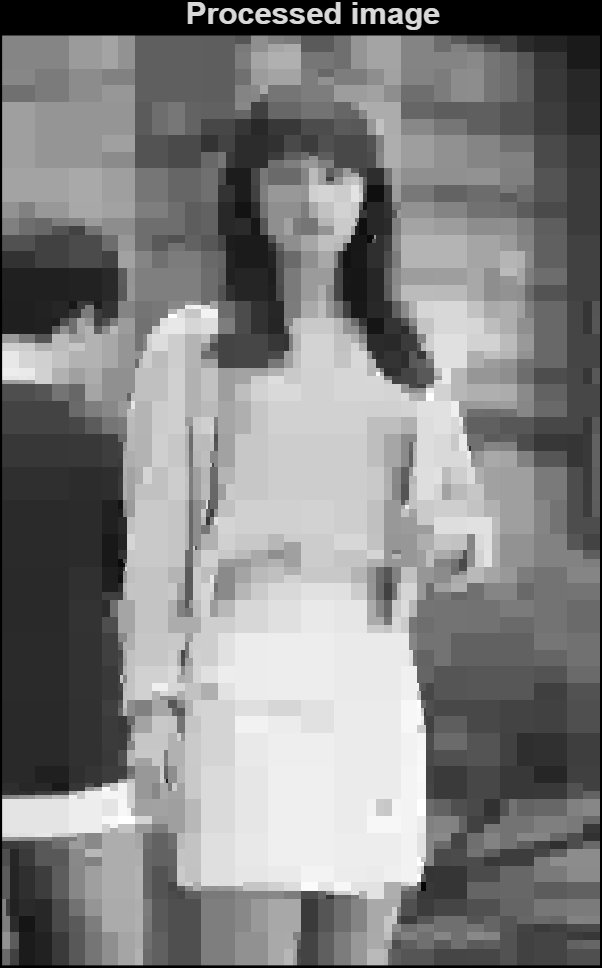
\includegraphics[width=\textwidth]{kjw1.png}
        \caption*{Người nổi tiếng}
    \end{subfigure}
    \hfill
    % Ảnh 2
    \begin{subfigure}[b]{0.24\textwidth}
        \centering
        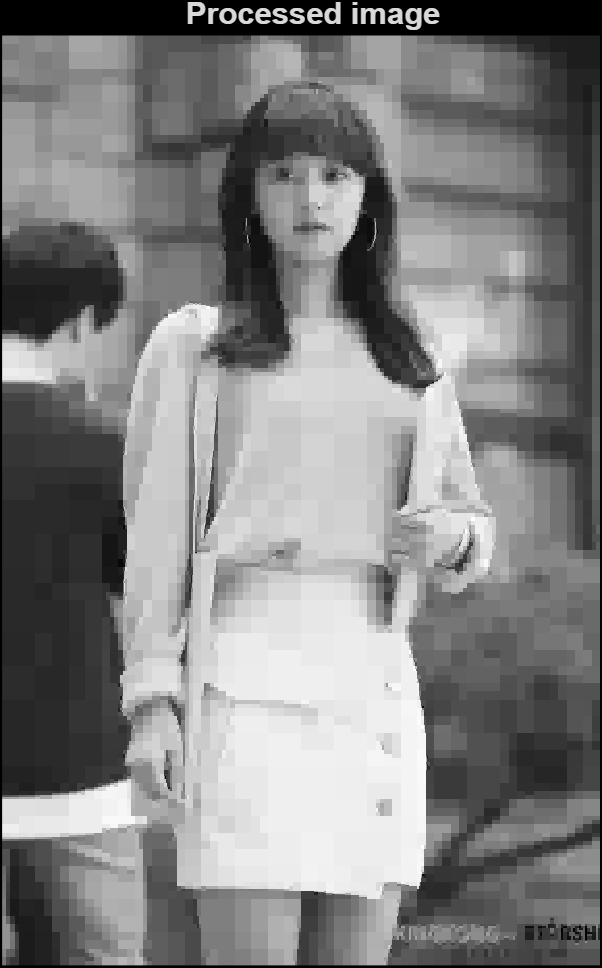
\includegraphics[width=\textwidth]{kjw2.png}
        \caption*{Người phụ nữ}
    \end{subfigure}
    \hfill
    % Ảnh 3
    \begin{subfigure}[b]{0.24\textwidth}
        \centering
        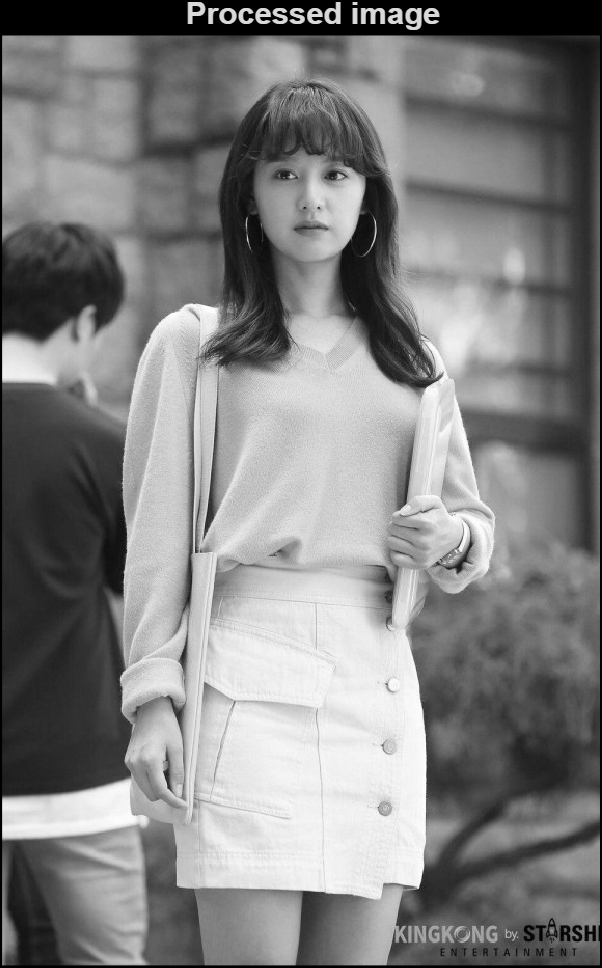
\includegraphics[width=\textwidth]{kjw3.png}
        \caption*{Diễn viên Kim Ji Won}
    \end{subfigure}
    \hfill

    \caption{Quá trình truyền tải hình ảnh.}
\end{figure}

\subsection*{2. Đối tượng và mục tiêu đề tài}

\textbf{Đối tượng nghiên cứu: } Đối tượng nghiên cứu của đề tài là phép biến đổi Haar (Haar Wavelet). Phép biến đổi sử dụng các ma trận trực giao để phân tích bức ảnh
thành các dải tần số thấp (chi tiết xấp xỉ) và các dải tần số cao (chi tiết độ nét, góc cạnh). Việc giữ lại phần xấp xỉ tổng thể và triệt tiêu một số chi tiết ta có thể thực hiện
nén một bức ảnh với dung lượng nhỏ hơn mà không gây ảnh hưởng quá nhiều đến chất lượng ảnh.

\vspace{0.3cm}
\noindent \textbf{Mục tiêu của đề tài bao gồm:}
\begin{itemize}
    \item Phân tích cơ sở lý thuyết đằng sau phép biến đổi Haar về mặt Đại số tuyến tính.
    \item Thực hiện quá trình nén ảnh và cắt ngưỡng (triệt tiêu một số chi tiết).
    \item Đánh giá hiệu năng và mức độ khôi phục hình ảnh của thuật toán.
\end{itemize}